\documentclass[12pt]{article}

% Input and configure the required packages.
% UCSD Mathematics Dissertation Template
%
% Please read the comments in this file and make appropriate edits.
% NOTE: Always refer to the ``Preperation and Submission Manual for
% Doctoral Dissertations and Masters Theses for 20**'', where 20** is
% the year of your graduation, for officiation preparations guidelines.
%
% If you desire more control, please see the attached files:
%   * ucsd.cls -- Class file
%   * uct10.clo, uct11.clo, uct12.clo -- Configuration files for font sizes 10pt,11pt,12pt
%
% CHANGELOG:
%   * Original file adapted from brockman.tex by JRB and RMR
%     to work with ucsd.cls

% Include all packages you need here.  Some standard options are suggested below.

% GEOMETRY - This will force the use of Letter paper.
% Many TeX installations default to A4 paper.  The formatting
% of the thesis class file requires Letter, else the margins
% will be wrong when you go to print it (and OGS will complain).
% If your TeX implementation is not setup for Letter paper, and
% you cannot change it, uncommenting the following line may fix
% problem.
% \usepackage[paper=letterpaper]{geometry}


%% AMS PACKAGES - Chances are you will want some or all of these if writing a math dissertation.
% \usepackage{amsmath, amscd, amssymb, amsthm}

%% GRAPHICX - This is the standard package for including graphics for latex/pdflatex.
% \usepackage{graphicx}

%% LATIN MODERN FONTS (replacements for Computer Modern)
% \usepackage{lmodern}
% \usepackage[T1]{fontenc}

%% INDEX
% Uncomment the following two lines to create an index:
% \usepackage{makeidx}
% \makeindex
% You will need to uncomment the \printindex line near the
% bibliography to display the index.  Use the command
% \index{keyword} within the text to create an entry in the index
% for keyword.

%% HYPERLINKS
% To create a PDF with hyperlinks, you need to include the hyperref package.
% THIS HAS TO BE THE LAST PACKAGE INCLUDED!
% Note that the options plainpages=false and pdfpagelabels exist
% to fix indexing associated with having both (ii) and (2) as pages.
% Also, all links must be black according to OGS.
% See: http://www.tex.ac.uk/cgi-bin/texfaq2html?label=hyperdupdest
% Note: This may not work correctly with all DVI viewers (i.e. Yap breaks).
% NOTE: hyperref will NOT work in draft mode, as noted above.
% \usepackage[colorlinks=true, pdfstartview=FitV, linkcolor=black, citecolor=black, urlcolor=black,plainpages=false,pdfpagelabels]{hyperref}
% \hypersetup{ pdfauthor = {Your Name Here}, pdftitle = {The Title of The Dissertation}, pdfkeywords = {Keywords for Searching}, pdfcreator = {pdfLaTeX with hyperref package}, pdfproducer = {pdfLaTeX}}

\usepackage{amsmath,amsfonts,amsthm,amssymb}
\usepackage{setspace}
\usepackage{fancyhdr}
\usepackage{lastpage}
\usepackage{extramarks}
\usepackage{chngpage}
\usepackage{soul}
\usepackage[usenames,dvipsnames]{color}
\usepackage{graphicx,float,wrapfig}
\usepackage{ifthen}
\usepackage{listings}
\usepackage{courier}
\usepackage[bw,framed,numbered]{mcode}
\usepackage{microtype}
\usepackage{appendix}
\usepackage{hyperref}
\usepackage[all]{hypcap}
\usepackage{url}

% Needed for changing the font size in \documentclass{} while
% using the fancyhdr package. Else the warning:
% \headheight is too small (12.0pt):Make it at least 14.49998pt.
\setlength{\headheight}{15pt}

% For faster processing, load Matlab syntax for listings
\definecolor{MyDarkGreen}{rgb}{0.0,0.4,0.0}
\lstloadlanguages{Matlab}%
\lstset{language=Matlab,
       frame=single,
       basicstyle=\scriptsize\ttfamily,
       keywordstyle=[1]\color{Blue}\bf,
       keywordstyle=[2]\color{Purple},
       keywordstyle=[3]\color{Blue}\underbar,
       identifierstyle=,
       commentstyle=\usefont{T1}{pcr}{m}{sl}\color{MyDarkGreen}\small,
       stringstyle=\color{Purple},
       showstringspaces=false,
       tabsize=5,
       % Put standard MATLAB functions not included in the default
       % language here
       morekeywords={xlim,ylim,var,alpha,factorial,poissrnd,normpdf,normcdf},
       % Put MATLAB function parameters here
       morekeywords=[2]{on, off, interp},
       % Put user defined functions here
       morekeywords=[3]{FindESS},
       morecomment=[l][\color{Blue}]{...},
       numbers=left,
       firstnumber=1,
       numberstyle=\tiny\color{Blue},
       stepnumber=0
       }

% Adds a hyperlink to an email address.
\newcommand{\mailto}[2]{\href{mailto:#1}{#2}}

% Homework Specific Information
\newcommand{\thesisTitle}{Master's Thesis}
\newcommand{\thesisSubTitle}{Robot Traffic School}
\newcommand{\thesisAuthorName}{Thomas Denewiler}
\newcommand{\thesisAuthorEmail}{tdenewiler@gmail.com}

% These commands set the document properties for the PDF output. Needs the hyperref package.
\hypersetup
{
    colorlinks,
    linkcolor={black},
    citecolor={black},
    filecolor={black},
    urlcolor={black},
    pdfauthor={\thesisAuthorName <\mailto{\thesisAuthorEmail}{\thesisAuthorEmail}>},
    pdfsubject={\thesisTitle},
    pdftitle={\thesisTitle},
    pdfkeywords={UC San Diego, Small Unmanned Ground Vehicles, Robotics},
    pdfstartpage={1},
}

% Includes a MATLAB script.
% The first parameter is the label, which also is the name of the script.
% The second parameter is the optional caption.
\newcommand{\matlabscript}[2]
  {\begin{itemize}\item[]\lstinputlisting[caption=#2,label=#1]{#1}\end{itemize}}

% User defined macros.
\def\argmin{\mathop{\arg\,\min}\limits}
\def\argmax{\mathop{\arg\,\max}\limits}
\def\argsol{\mathop{\arg\,\text{sol}}\limits}


% Document starts here.
\begin{document}
\title{Notes on Lyapunov Controller}
\author{Thomas Denewiler}
\maketitle

% Meat and potatoes.
\section{Control Law}
\begin{align*}
u &= \gamma e\cos\alpha \\
\omega &= k\alpha + \gamma\frac{\cos\alpha\sin\alpha}{\alpha}\left(\alpha+h\theta\right)
\end{align*}

\begin{figure}[ht!]
	\centering
	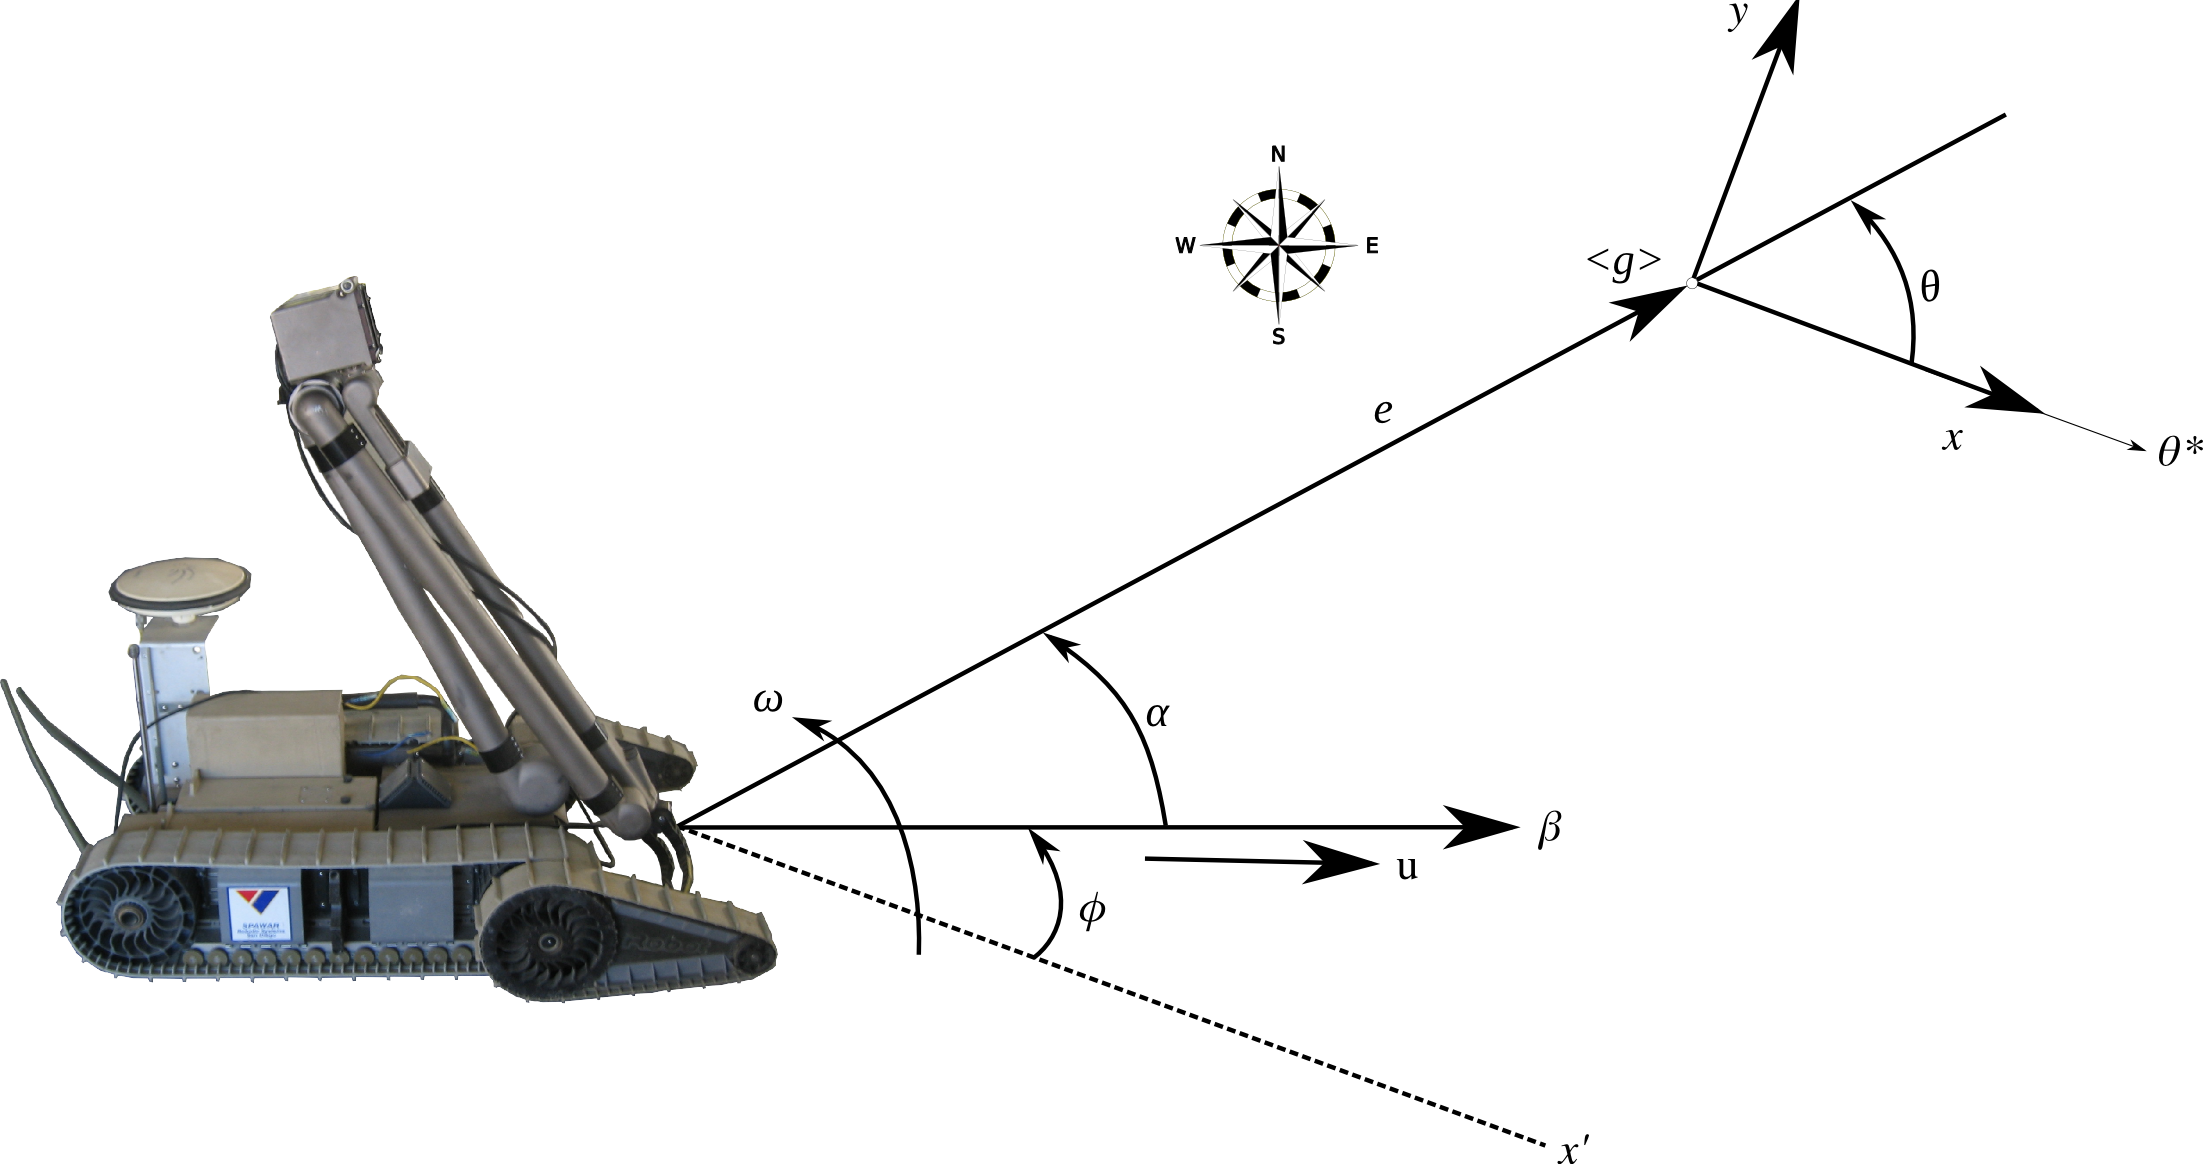
\includegraphics[width=.95\textwidth]{images/packbotlyapunov}
	\caption{PackBot with coordinate system for the Lyapunov controller.}
	\label{fig:pblyapunov}
\end{figure}

\section{Variables}
\begin{table}[ht!]
\caption{Variables needed for Lyapunov controller.}
\small
\centering
\begin{tabular}{@{}lllr@{}} \toprule
Description                   & Figure         & Units   & Range \\ \midrule
Distance error                & $e$            & meters  & N/A \\
Robot heading                 & $\psi$         & radians & $(-\pi,\pi]$ \\
Goal heading                  & $\theta^\star$ & radians & $(-\pi,\pi]$ \\
Heading error                 & $\theta$       & radians & $(-\pi,\pi]$ \\
Heading error - robot heading & $\alpha$       & radians & $(-\pi,\pi]$ \\
Goal heading - robot heading  & $\phi$         & radians & $(-\pi,\pi]$ \\ \bottomrule
\end{tabular}
\label{tab:LyapunovVariables}
\end{table}

The way to calculate the variables is:
\begin{enumerate}
\item $dx$ is the vertical component of the error vector $e$ since the $x-$axis is forward of the vehicle as seen in Figure \ref{fig:pblyapunov}.
\item $dy$ is the horizontal component of the error vector $e$ as seen in Figure \ref{fig:pblyapunov}.
\item $e$ can be calculated in several different ways:
\begin{itemize}
\item Use \texttt{Path\_Executor()} to set a carrot out front of the robot on the path. The carrot moves out along the next path segment when the robot gets close enough to the end waypoint of the current path segment. This could cause $e$ to be much smaller than it actually is so $\alpha$ will be corrected before it should be and a problem could occur if the robot tries to correct $\theta$ too early.
\item Use \texttt{sqrt(pow(dx,2) + pow(dy,2))} to get the distance to the end waypoint on the current path segment. This will cause the robot to slow down as it reaches every waypoint, even intermediate ones. Conversely, if $e$ is very large then $u$ could grow to be too large as well and necessitate the use of a limiting value for $u$.
\item Combine the two methods and use the actual distance to the end waypoint of the current path segment until that value is less than the distance to the carrot and then use the carrot distance for $e$.
\end{itemize}
\item $\psi$ is the current heading of the robot in the world coordinate frame and ends up being \texttt{globalPose.yaw} from \texttt{PBGlobalWaypointDriver} which is available from the \texttt{Get\_Heading()} function.
\item $\alpha$ is the angle between the current heading of the robot $\psi$ and the error vector $e$ where the angle of the error vecotr $e$ is from the current position to the waypoint and found as $\tan^{-1}\left(\frac{dy}{dx}\right)$. The desired angle error is $\alpha = \tan^{-1}\left(\frac{dx}{dy}\right) - \psi$.
\item $\theta^\star$ is the desired heading in the global coordinate system and there are multiple ways that it \textit{could} be set.
\begin{itemize}
\item $\theta^\star=0$ would just make the desired heading be North.
\item $\theta^\star=\psi$ would make the desired heading be the same as whatever the current heading happens to be.
\item It could be sent in as part of a waypoint, say from MOCU via JAUS.
\item Look at the current waypoint and next waypoint positions. If there is no next waypoint then just go straight to the current waypoint with $\theta^\star=\psi$. If there is a next waypoint then the $\theta^\star$ could be the angle from the current waypoint to the next waypoint or splitting the difference between heading to the current and next waypoints.
\end{itemize}
\item $\phi=\theta^\star-\psi$.
\item $\theta=\alpha + \phi$.
\end{enumerate}
Don't forget that all of the angle variables need to be normalized so that they are in the range $(-\pi,\pi]$.

\section{Effect of Gains on Angular Velocity}
The most important item to note is that when driving a PackBot (and many other differential drive vehicles) $\omega>0\Rightarrow$ \textit{turn left} and $\omega<0\Rightarrow$ \textit{turn right}. This is a consequence of how the $x-$, $y-$ and $z-$axes are defined as in Figure \ref{fig:packbotaxes}. It can be seen that the positive $x-$axis is forward of the vehicle and the positive $y-$axis is left of the vehicle. Following the right-hand rule the $z-$axis is required to be positive in the up direction and that positive rotations about the $z-$axis (or changes in yaw due to the angular velocity command) move from the positive $x-$axis to the positive $y-$axis.

It is also helpful to rewrite the angular velocity output from the control law as
\begin{align*}
\omega = k\alpha + \gamma\cos\alpha\sin\alpha + \frac{\gamma h\theta\cos\alpha\sin\alpha}{\alpha}
\end{align*}

\begin{figure}[ht!]
	\centering
	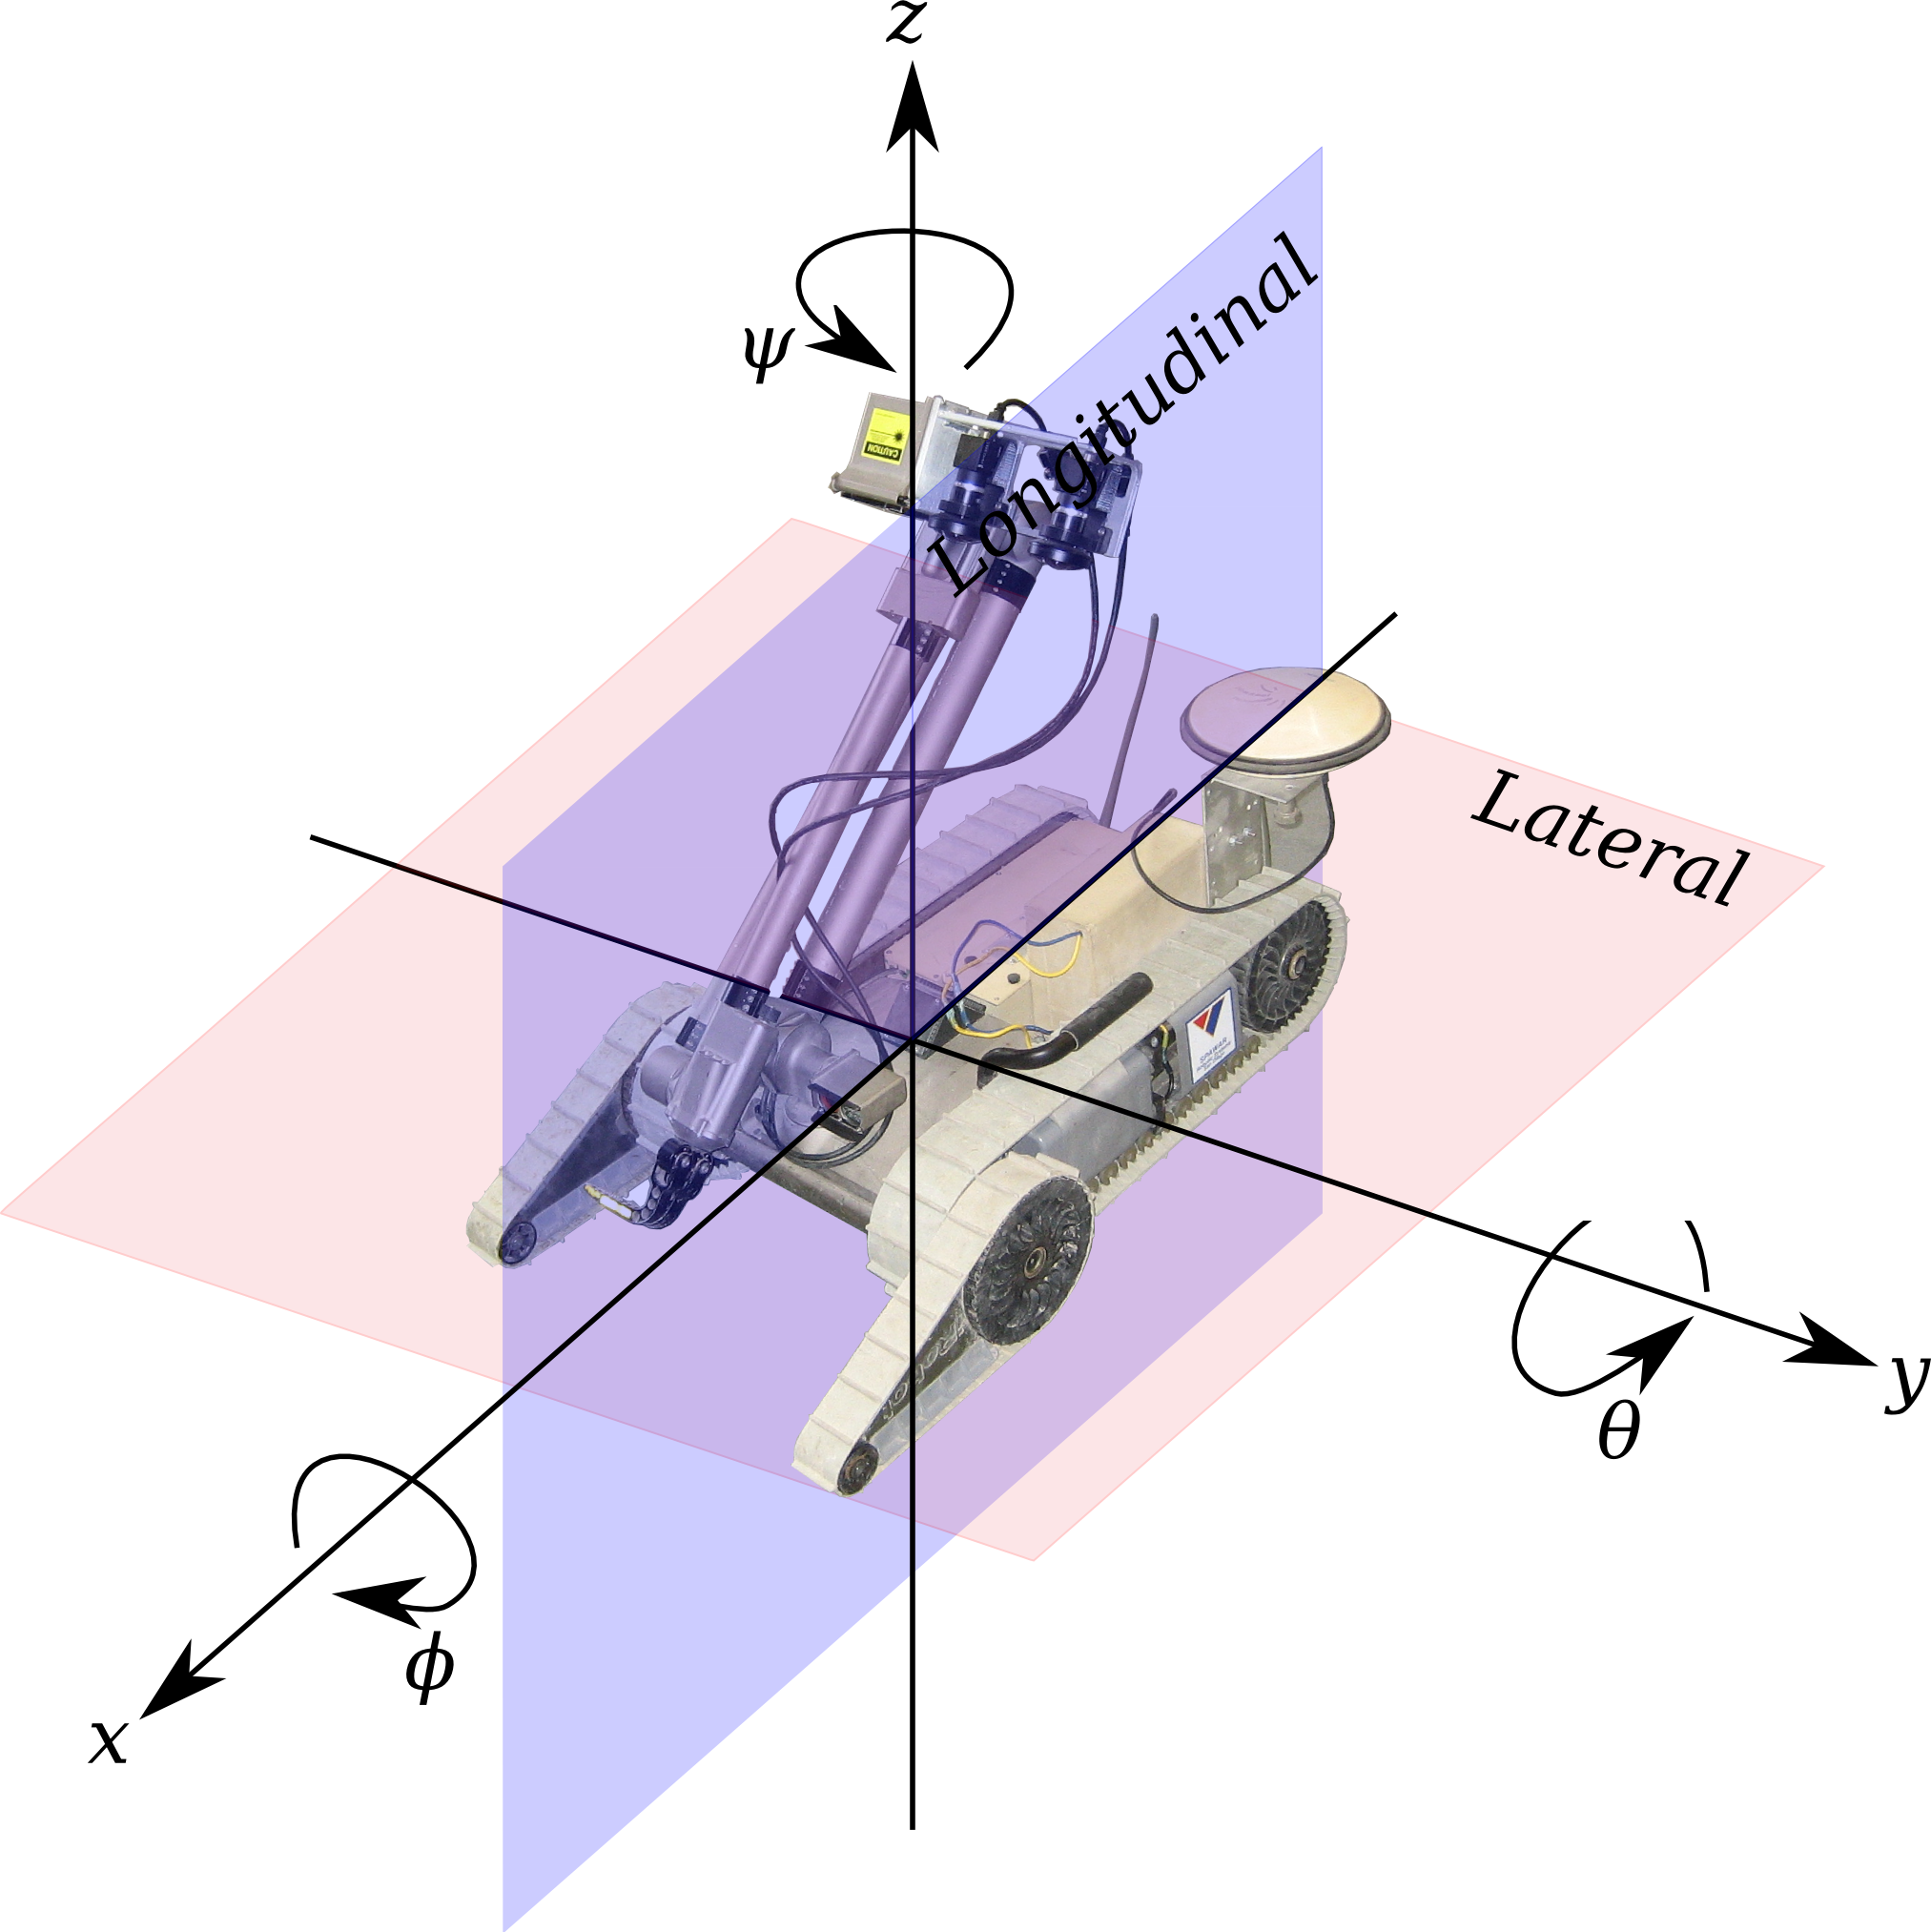
\includegraphics[width=.5\textwidth]{images/packbotaxes}
	\caption{Body centered coordinate frame for PackBot.}
	\label{fig:packbotaxes}
\end{figure}

There are three gains that affect the angular velocity output: $h$, $k$ and $\gamma$. The gains are all coupled in a nonlinear fashion so it can be difficult to intuitively understand how the angular velocity output will change as the gains are modified. In ACS angles are defined to be in the range $(-\pi,\pi]$ as well and Figure \ref{fig:plotSinCos} shows several useful trigonometric functions of $\alpha$ in the range of interest.

\begin{figure}[ht!]
	\centering
	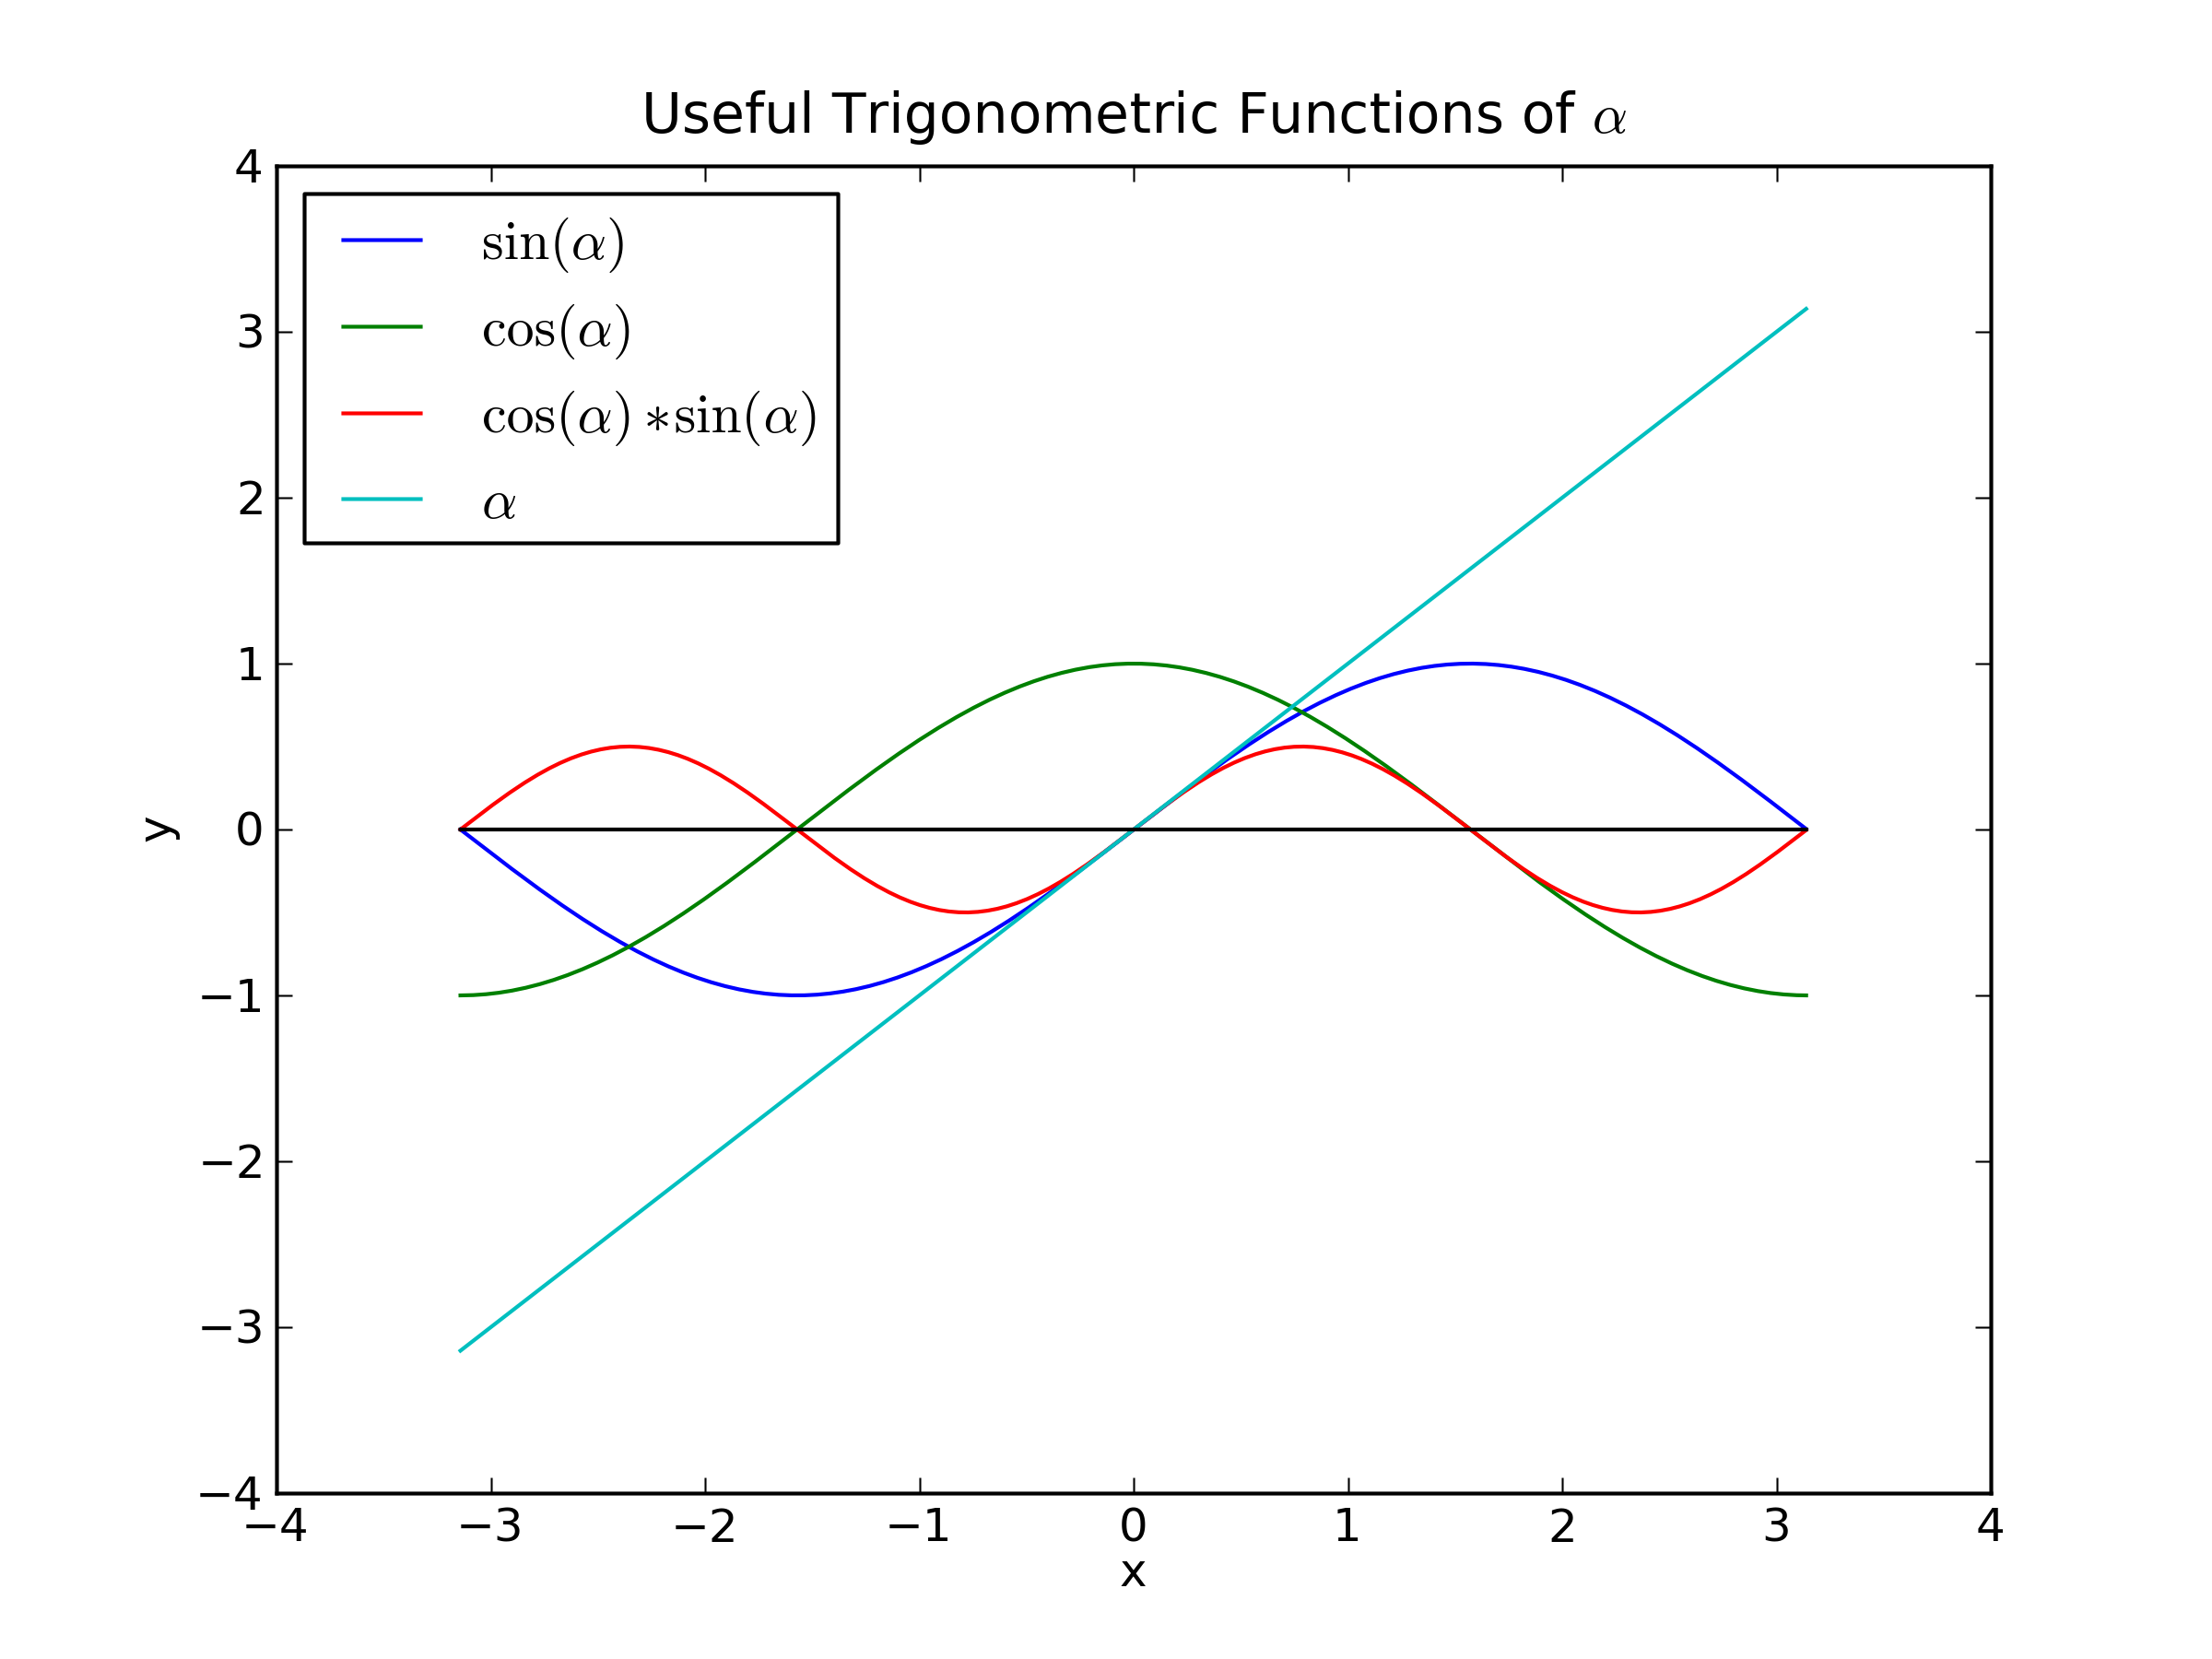
\includegraphics[width=.75\textwidth]{images/plotSinCos}
	\caption{Plot of $\alpha$, $\sin\alpha$, $\cos\alpha$ and $\sin\alpha*\cos\alpha$.}
	\label{fig:plotSinCos}
\end{figure}

When looking at the angular velocity output and the gains there are thirteen combinations that can be used when setting the gain values relative to each other as shown in Table \ref{tab:gainsAngVelOutput}. Note that when two variables are larger than one variable some terms cancel out as the effects of the term with the smaller gain value diminish. The gains also have different effects depending on which quadrant $\alpha$ and $\theta$ are in as shown for $\alpha$ in Figure \ref{fig:robotAlpha}.

\begin{figure}[ht!]
	\centering
	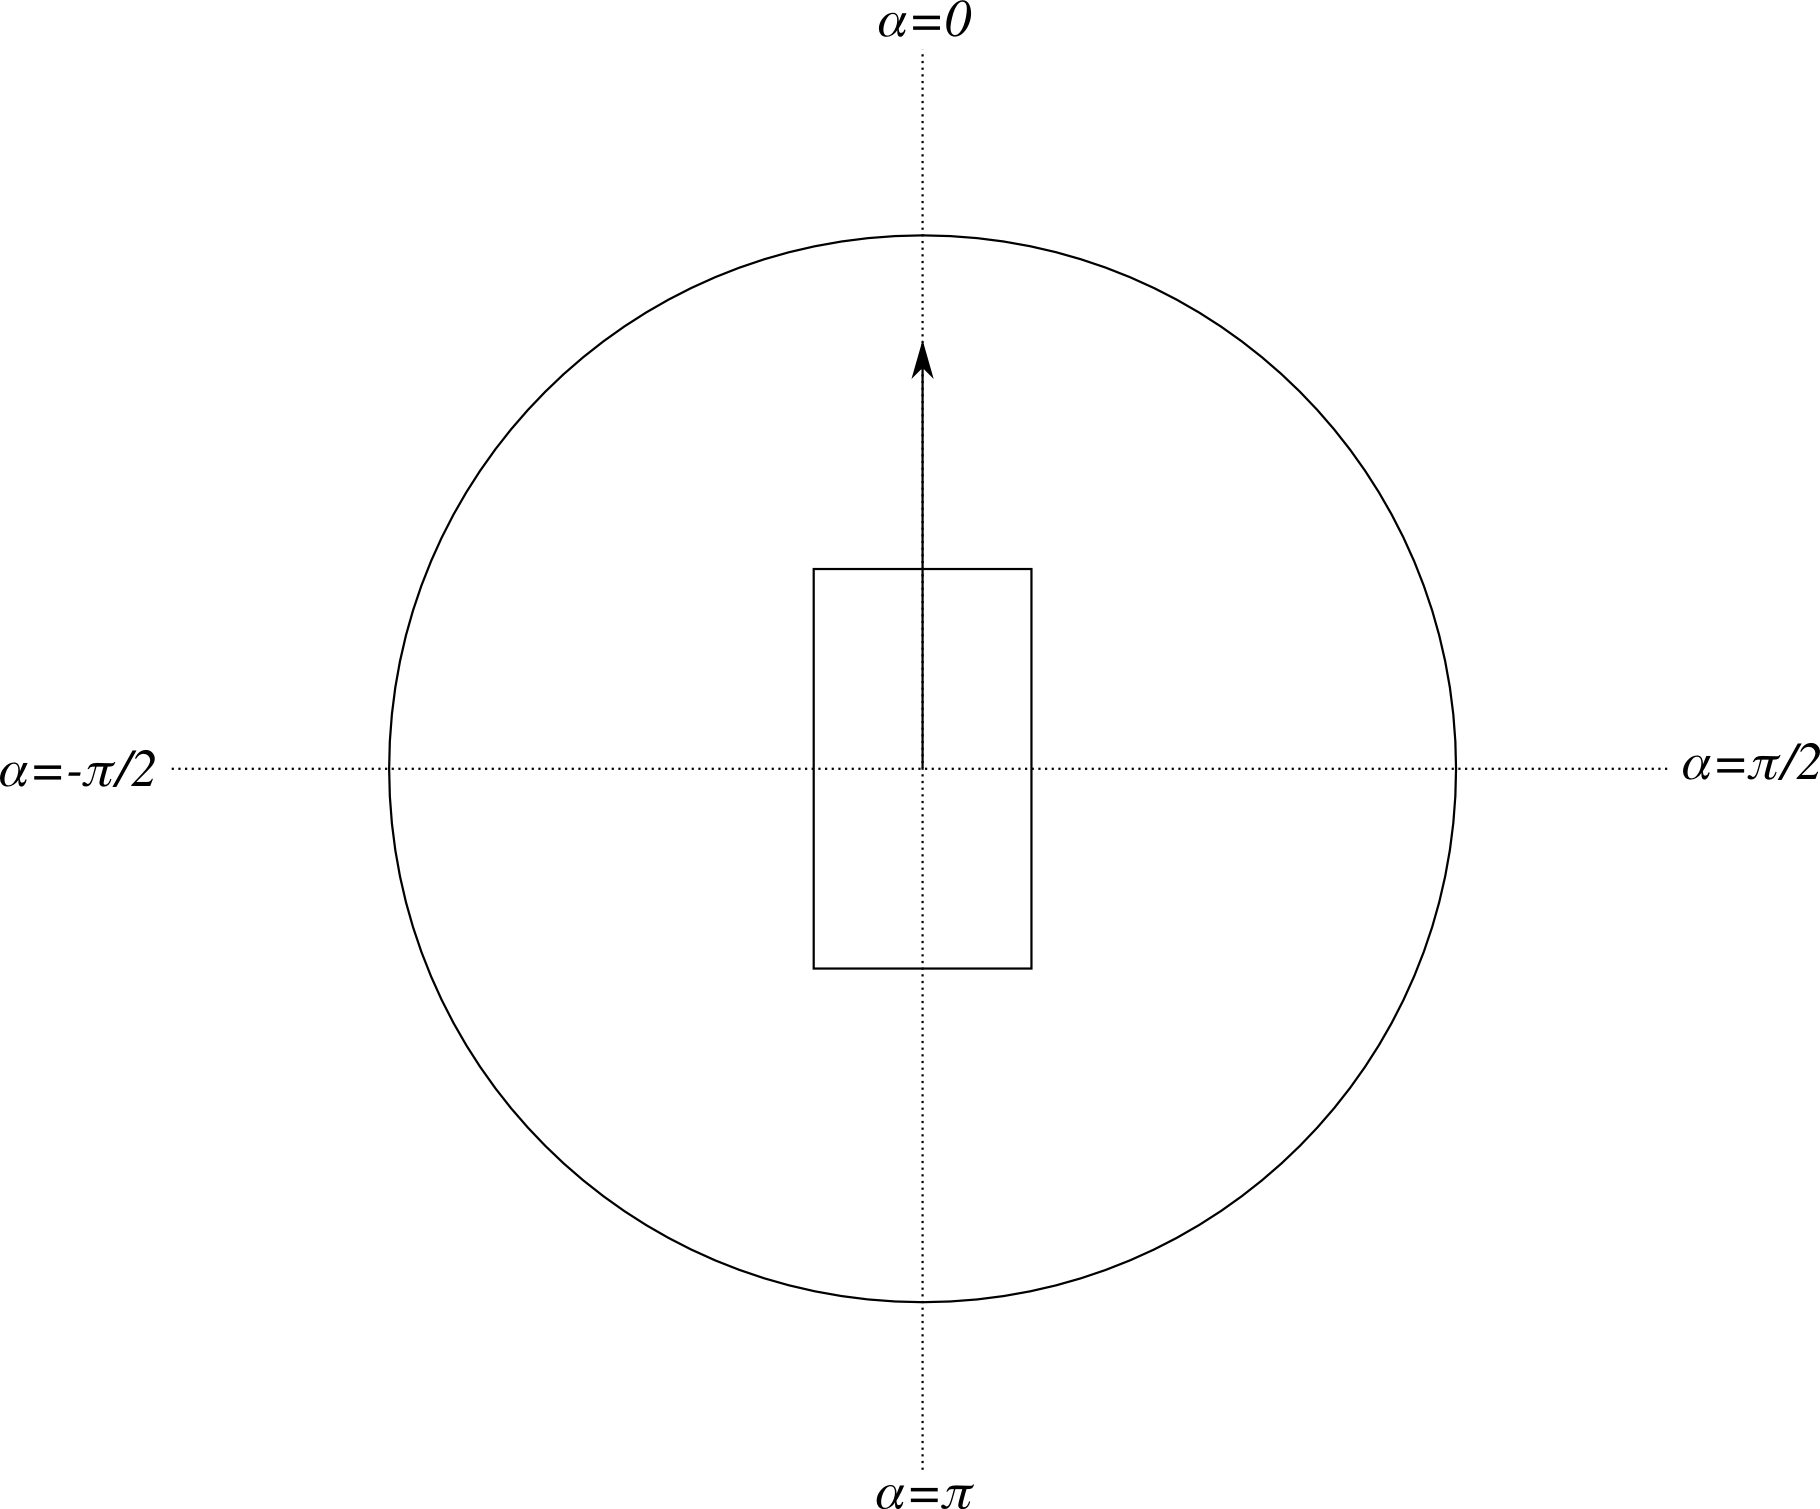
\includegraphics[width=.3\textwidth]{images/robotAlpha}
	\caption{Different $\alpha$ values for varying target positions.}
	\label{fig:robotAlpha}
\end{figure}

\begin{table}[ht!]
\caption{Gains and angular velocity output.}
\small
\centering
\begin{tabular}{@{}llr@{}} \toprule
Scenario & Gains                     & Angular Velocity $\omega$ \\ \midrule
1        & $h\approx k\approx\gamma$ & $\omega\approx k\alpha + \gamma\cos\alpha\sin\alpha + \gamma h\theta\cos\alpha\sin\alpha/\alpha$ \\
2        & $k\gg h,\gamma$           & $\omega\approx k\alpha$ \\
3        & $\gamma\gg h,k$           & $\omega\approx \gamma\cos\alpha\sin\alpha$ \\
4        & $h,k \gg\gamma$           & $\omega\approx k\alpha\cancelto{0}{+\gamma h\theta\cos\alpha\sin\alpha/\alpha}$ \\
5        & $h,\gamma\gg k$           & $\omega\approx \cancelto{0}{\gamma\cos\alpha\sin\alpha+} \gamma h\theta\cos\alpha\sin\alpha/\alpha$ \\
6        & $k,\gamma\gg h$           & $\omega\approx k\alpha + \gamma\cos\alpha\sin\alpha \cancelto{0}{+\gamma h\theta\cos\alpha\sin\alpha/\alpha}$ \\
7        & $h\gg k,\gamma$           & $\omega\approx \gamma h\theta\cos\alpha\sin\alpha/\alpha$ \\
8        & $h\gg k\gg\gamma$         & $\omega\approx \gamma h\theta\cos\alpha\sin\alpha/\alpha$ \\
9        & $h\gg\gamma\gg k$         & $\omega\approx \gamma h\theta\cos\alpha\sin\alpha/\alpha$ \\
10       & $k\gg h\gg\gamma$         & $\omega\approx k\alpha$ \\
11       & $k\gg\gamma\gg h$         & $\omega\approx k\alpha$ \\
12       & $\gamma\gg h\gg k$        & $\omega\approx \gamma\cos\alpha\sin\alpha$ \\
13       & $\gamma\gg k\gg h$        & $\omega\approx \gamma\cos\alpha\sin\alpha$ \\ \bottomrule
\end{tabular}
\label{tab:gainsAngVelOutput}
\end{table}

\end{document}
